\documentclass[a4paper,12pt,oneside]{article}
\usepackage{amsmath}
\usepackage{amssymb}
\usepackage[colorlinks]{hyperref}
\usepackage{graphicx}
\usepackage{enumitem}
\usepackage[utf8]{inputenc}
\usepackage[croatian]{babel}


\usepackage{blindtext}
\usepackage{geometry}
\geometry{
	a4paper,
	total={170mm,257mm},
	left=15mm,
	top=15mm,
	bottom=15mm,
	right=15mm
}


\usepackage{multirow}

\usepackage{listings}
\usepackage{xcolor}

\definecolor{codegreen}{rgb}{0,0.6,0}
\definecolor{codegray}{rgb}{0.5,0.5,0.5}
\definecolor{codepurple}{rgb}{0.58,0,0.82}
\definecolor{backcolour}{rgb}{0.95,0.95,0.92}

\newcommand{\ceil}[1]{\lceil {#1} \rceil}

\lstdefinestyle{mystyle}{
	backgroundcolor=\color{backcolour},   
	commentstyle=\color{codegreen},
	keywordstyle=\color{magenta},
	numberstyle=\tiny\color{codegray},
	stringstyle=\color{codepurple},
	basicstyle=\ttfamily\footnotesize,
	breakatwhitespace=false,         
	breaklines=false,                 
	captionpos=b,                    
	keepspaces=true,                 
	numbers=left,                    
	numbersep=2pt,                  
	showspaces=false,                
	showstringspaces=false,
	showtabs=false,                  
	tabsize=1
}

\lstset{style=mystyle}

\title{Kriptografija i sigurnost mreža 2023.}
\author{ 2. domaća zadaća \\ Doris Đivanović } 
\date{}
\begin{document}
	\maketitle
 	\pagenumbering{gobble} 
\section*{Zadatak 1}
\textbf{Vigenereovom širom} iz otovorenog tetksta na hrvatskom jeziku dobiven je šifrat:

\begin{table}[h!]
\begin{tabular}{lllllllll}
RZZRU & VXCAM & ZEAXH & EXGTB & SMYUX & NUVYI & AWMIO & ZQFHW & \\
OVJHI & IIAYB & ZTUVX & XDWTI & GOYZU & JZFHT & ZOACF & MPEHO & \\
RXGVA & XZPOS & JGHJG & RHYDE & RFPPD & XKTPY & NHGSJ & BZOUN & \\
ZZIYI & NTFHN & KCXRN & HGVPZ & HTXED & GSERA & HZNZG & AATZF & KTP \\
\end{tabular}
\end{table}

\noindent Odredite najprije \textbf{duljinu ključne riječi}, potom samu \textbf{ključnu riječ}, te
\textbf{dekriptirajte šifrat}.	

\section*{Duljina ključne riječi}
\subsection*{Prva metoda}
Duljinu ključne riječi najprije sam pokušala odrediti pomoću tzv. \textbf{Kasiskijevog testa}. Vrlo brzim pregledom šifrata uočila sam da je jedini trigram koji se u šifratu pojavljuje dva puta \textbf{UVX}. Četvrto slovo jednog i drugog trigrama ne podudaraju se, pa zaključujem da u šifratu sigurno nema segmenata duljine veće od 3 koji se pojavljuju dva puta. Trigram UVX prvi se put pojavljuje na poziciji 5, a drugi put na poziciji 53, pa razlika njihovih pozicija iznosi $53 - 5 = 48$. Broj 48 možemo faktorizirati na sljedeće načine: $48 = 2^4 \cdot 3 = 16 \cdot 3 = 8 \cdot 6$. Među višekratnicima ove razlike mogu pronaći neke kandidate za duljinu ključne riječi, pa bih mogla pretpostaviti da je duljina ključne riječi $m = 3$ (iako mi je to sumnjivo), ili možda $m = 6$.
\subsection*{Druga metoda}
Pribjegavam drugoj metodi koja za svaki kandidat $m$ za duljinu ključne riječi dani šifrat zapisuje stupac po stupac  u (krnju) matricu dimenzija $m \times \ceil{m/n}$, gdje je $n$ duljina šifrata. Time šifrat dijeli u $m$ podnizova, koji su pojedinačno, ako je $m$ uistinu duljina ključne riječi, šifrirani Cezarovom šifrom s nekim ključem. Također, tada \textbf{indeks koincidencije} svakog od podnizova mora biti \textbf{jako blizu 0.064} (\underline{$\approx 0.064$ ima tekst pisan na govornom jeziku, a i njegov monoalfabetski šifrat}).

Napisala sam sljedeći program koji taj postupak radi za $m = 1, 2, \dots, 10$. Za svaki $m$ kreira se i na ekran ispisuje matrica. "Višak u matricama" popunila sam znakom *. Zatim se za svaki podniz $z_1, \dots, z_m$ računa indeks koincidencije $I_c(z_i)$ po formuli i ispisuje se na ekran. Radi lakše provjere koji je $m$ vjerojatnije duljina ključne riječi, za svaki dobiveni indeks računala sam i ispisala njegovo odstupanje od broja 0.064 - u kodu nazvano \textbf{GREŠKA}.

\lstinputlisting[language=C++]{VigenereDuljina.cpp}

\subsection*{Druga metoda - analiza rezultata}
Gledajući output dobiven na ekranu, čini mi se da su najmanje greške za $m = 3$ i $m = 6$, ali još ne mogu zaključiti koja je sigurno duljina ključne riječi:

\begin{figure}[h!] %h! za objekte koje UBACUJEMO u sve, za plutajuće objekte, slike i tablice
	\centering
		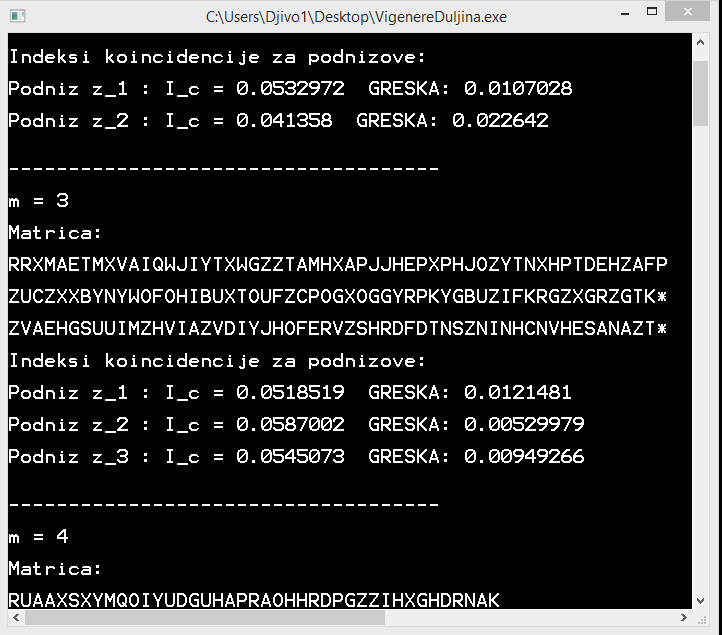
\includegraphics[width=0.57\textwidth]{output1.png}  
%	\caption{Dio outputa gdje se vide indeksi koincidencije za m = 3} 
\end{figure}

\newpage

\begin{figure}[h!] %h! za objekte koje UBACUJEMO u sve, za plutajuće objekte, slike i tablice
	\centering
	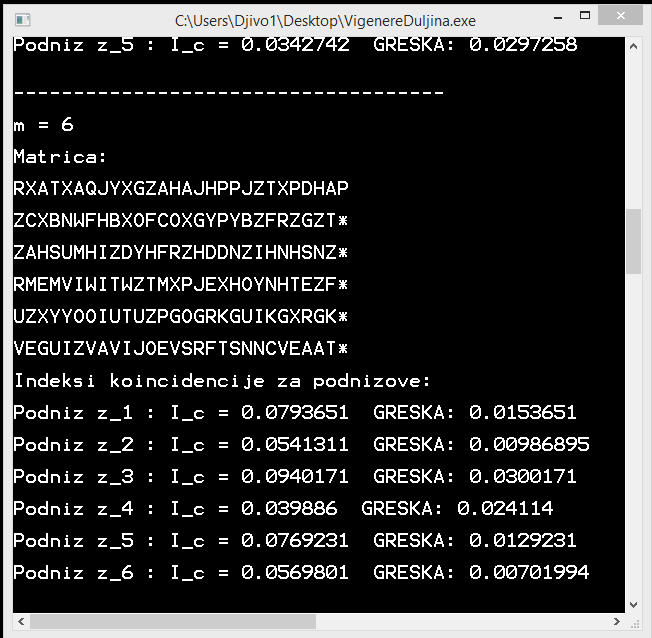
\includegraphics[width=0.57\textwidth]{output2.png} 
	%	\caption{Dio outputa gdje se vide indeksi koincidencije za m = 6}  
\end{figure}
\section*{Ključna riječ}
U svrhu određivanja same ključne riječi, napisala sam još jedan program. On nam omogućava da za fiksiranu, odabranu duljinu ključne riječi $m$ odredimo ključnu riječ. Program najprije fiksira $m$. Zatim kreira i ispisuje na ekran gore spomenutu matricu samo za tu duljinu. Zatim, postupkom koji smo radili na predavanju, pretpostavljajuči da je \textbf{otvoreni tekst pisan na hrvatskom jeziku}, računamo zajedničke indekse koincidencije svakog od podnizova $z_1, \dots, z_m$, tj. svakog retka matrice $j = 1, \dots, m$, i slučajnog teksta na hrv. jeziku, i time za svaki redak računamo ključ $k_j$ za njegovu Cezarovu šifru. Na kraju, spajanjem tih ključeva u jedan, tj. u jednu riječ, dobivamo i ispisujemo na ekran ključnu riječ duljine $m$ za Vigenereovu šifru. Također, prolazeći po retcima matrice, dešifriramo svaki redak njegovim ključem i dešifrirane elemente spremamo na odgovarajuća mjesta. Dešifriranu matricu ispisujemo kao jedan string prolazeći po stupcima i time dobivamo otvoreni tekst za tu ključnu riječ.

\lstinputlisting[language=C++]{VigenereKljuc.cpp}

\textbf{Uočimo da nam ovaj program može poslužiti kao konačan alat za određivanje duljine ključne riječi}. Jednostavno, mijenjanjem parametra $m$, možemo vidjeti za koji će dobivena ključna riječ biti smislena (iako to ne mora biti), ali možemo vidjeti i za koji će $m$ otvoreni tekst biti smislena poruka, što nam je sigurna potvrda.
Uvrštavanjem $m = 3$ u gornji program, dobiva se da je ključna riječ = PGZ, a otvoreni tekst uopće nije smislen. Međutim, uvrštavanjem $m = 6$, dobiva se da je ključna riječ = POŽEGA i dobiva se smisleni otvoreni tekst:
 
\begin{figure}[h!] %h! za objekte koje UBACUJEMO u sve, za plutajuće objekte, slike i tablice
	\centering
	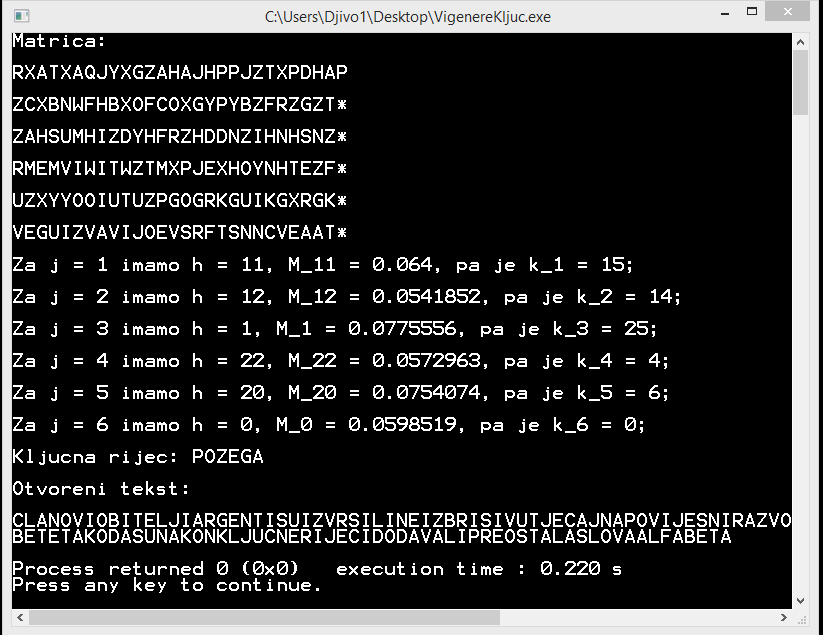
\includegraphics[width=0.57\textwidth]{OUTPUT3.png}  
	%	\caption{Output programa}  
\end{figure}

Dakle, zaključujemo da je:
\begin{itemize}
\item \textbf{duljina ključne riječi = 6},
 
\item\textbf{ključna riječ = POŽEGA},
  
\item \textbf{otvoreni tekst} glasi:
\end{itemize}
\textbf{CLANOVI OBITELJI ARGENTI SU IZVRSILI NEIZBRISIV UTJECAJ NA POVIJESNI RAZVOJ KRIPTOLOGIJE. SASTAVLJALI SU SIFARSKE ALFABETE TAKO DA SU NAKON KLJUCNE RIJECI DODAVALI PREOSTALA SLOVA ALFABETA.}

\newpage
\section*{Zadatak 2}
Šifrirajte otvoreni tekst 
\begin{center}
PARKER HITT
\end{center}
\noindent pomoću \textbf{Playfairove šifre} s ključnom riječi CRYPTOGRAPHY.
\subsection*{Rješenje}
\noindent Matrica slova dimenzije $5 \times 5$ uzimajući u obzir ključnu riječ:
\begin{table}[h!]
	\centering
	\begin{tabular}{ccccc}
		C & R & Y & P & T \\
		O & G & A & H & B \\
		D & E & F & IJ & K \\
		L & M & N & Q & S \\
		U & V & W & X & Z \\
	\end{tabular}
\end{table}

\noindent Rastav otvorenog teksta na bigrame:
\begin{center}
	 PA  RK  ER  HI  TT
\end{center}
Bigram od istih slova rastavlja se s X, broj slova do parnog nadopunjuje se s X:
\begin{center}
	PA  RK  ER  HI  TX  TX
\end{center}
Šifriranje:
\begin{itemize}
	\item P i A nasuprotni vrhovi pravokutnika $\Rightarrow$ PA $\rightarrow$ YH,
	\item R i K nasuprotni vrhovi pravokutnika $\Rightarrow$ RK $\rightarrow$ TE,
	\item E i R u istom stupcu $\Rightarrow$ ER $\rightarrow$ MG,
	\item H i I u istom stupcu $\Rightarrow$ HI $\rightarrow$ IQ,
	\item T i X nasuprotni vrhovi pravokutnika $\Rightarrow$ TX $\rightarrow$ PZ.
\end{itemize}
\textbf{Šifrat:}
\begin{center}
		\textbf{YHTEMG  IQPZPZ}
\end{center}

\newpage
\section*{Zadatak 3}
Odredite ključ $K$ u \textbf{Hillovoj šifri} ako je poznato da je $m = 2$, te da
otvorenom tekstu
\begin{center}
HEBERN
\end{center}
odgovara šifrat
\begin{center}
RVBHCF.
\end{center}
\subsection*{Rješenje}
Budući da je $m = 2$, Hillovom se šifrom dva uzastopna slova u otvorenom tekstu zamjenjuju s dva uzastopna slova u šifratu. Stoga, kako znamo da se otvoreni tekst HEBERN šifrira u RVBHCF, uz tablicu korespondencije slova međunarodne abecede i skupa ostataka modulo $26$, možemo zaključiti da za traženi ključ $K$ vrijedi:
\begin{align*}
	&e_K(7, 4) = (17, 21), \\
	&e_K(1, 4) = (1, 7), \\
	&e_K(17, 13) = (2, 5). \\
\end{align*}
Dakle, imamo tri para uređenih parova
$$(x_{1j}, x_{2j}) \quad \text{i} \quad (y_{1j}, y_{2j}) \quad \text{t. d.} \quad e_K(x_{1j}, x_{2j}) = (y_{1j}, y_{2j}). $$
Budući da je $m = 2$, za analizu su nam dovoljna dva uređena para, npr. $(7, 4)$ i $(17, 13)$.
Iz gornjih dviju  jednadžbi te definicije Hillovog kriptosustava dobivamo sljedeću matričnu jednadžbu (\textbf{sve operacije su mod $26$}):
$$\left|\begin{matrix} 7 & 4 \\
	                   17 & 13 \\ \end{matrix}\right| K = \left|\begin{matrix} 17 & 21 \\
	                  2 & 5 \\ \end{matrix}\right| .$$
Ako je matrica $X$ invertibilna, ključ $K$ možemo dobiti na sljedeći način:
$$K = X^{-1}Y.$$
Znamo da je matrica $A$ u $\mathbb{Z}_{26}$ invertibilna akko joj je determinanta invertibilna u $\mathbb{Z}_{26}$, tj. ako je $(\text{det}A, 26) = 1$, i tada je
$$A^{-1} = (\text{det}A)^{-1}\left|\begin{matrix} a_{22} & -a_{12} \\
	-a_{21} & a_{11} \\ \end{matrix}\right| .$$
Računamo
$$\text{det}X = \text{det}\left|\begin{matrix} 7 & 4 \\
	17 & 13 \\ \end{matrix}\right| = 7 \cdot 13 - 17 \cdot 4 = 91 - 68 = 23 \ \text{mod} \ 26  = 23.$$
Sada iz tablice inverza u $\mathbb{Z}_{26}$
\begin{table}[h!]
\begin{tabular}{cccccccccccc}
	1 & 3 & 5 & 7 & 9 & 11 & 15 & 17 & 19 & 21 &
	23 & 25  \\
	1 & 9 & 21 & 15 & 3 & 19 & 7 & 23 & 11 & 5 &
	17 & 25  \\
\end{tabular}
\end{table}


\noindent vidimo da je 
$$(\text{det}X)^{-1} = 23^{-1} = 17,$$
pa je $X$ invertibilna matrica i vrijedi
$$X^{-1} = 17\left|\begin{matrix} 13 & -4 \\
	-17 & 7 \\ \end{matrix}\right| = \left|\begin{matrix} 13 & 10 \\
	23 & 15 \\ \end{matrix}\right|$$
Konačno, \textbf{možemo izračunati ključ} $K$:
$$K = \left|\begin{matrix} 13 & 10 \\
	23 & 15 \\ \end{matrix}\right|\left|\begin{matrix} 17 & 21 \\
	2 & 5 \\ \end{matrix}\right| = \left|\begin{matrix} 7 & 11 \\
	5 & 12 \\ \end{matrix}\right|.$$
Za kraj ćemo provjeriti odgovara li dobiveni ključ $K$ informaciji
$$e_K(1, 4) = (1, 7).$$
Dobivamo:
$$e_K(1, 4) = (1, 4)K = (1, 4)\left|\begin{matrix} 7 & 11 \\
	5 & 12 \\ \end{matrix}\right|  =  (1, 7),$$
dakle u redu je.
\end{document}
